\documentclass{article}
\author{Group 16}
\usepackage{float}
\usepackage{graphicx}
\usepackage{subfigure}
\usepackage{geometry}
\usepackage{titlesec}
\usepackage{fancyhdr}
\usepackage{enumitem}
\usepackage{listings}
\usepackage{xcolor}
\usepackage{array}
\usepackage{mathtools}
\usepackage{float}
\usepackage{indentfirst}
\usepackage{multirow}
\usepackage{subfigure}
\usepackage{listings}
\usepackage{lmodern}
\usepackage{amssymb}
\usepackage{booktabs}
\geometry{top=1in,bottom=1in,left=1in,right=1in}
\linespread{1.2}

% \title{Aynalysis of audio source separation}
\begin{document}
    % \maketitle
    \begin{center}   
        \huge 
        \textbf{Audio Source Separation Report}\\
        \normalsize{Group 16}
    \end{center}

    \normalsize
    \section{Algorithm Analysis}
        \subsection{AoA Estimation}
            The AoA Estimation is based on the Delay-and-Sum Algorithm which has been described in the lab document and will not be repeated here.
            % \begin{figure}[H]
            %     \centering
            %     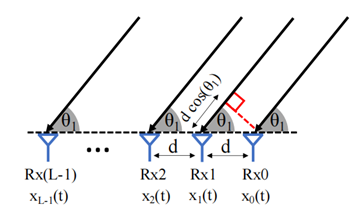
\includegraphics[width = 0.3\textwidth]{pic/fig1.png}
            %     \caption{AoA estimation with Linear Array}
            % \end{figure}

            % Now note that the signal arriving at antenna k, that is $x_k(t)$ is simply a delayed version of $x_0(t)$, since to reach antenna k the signal has to travel an additional distance of $kdcos(\theta_1)$. Hence we have 

            % $$
            % x_k(t) = x_0 (t -dcos(\theta_1)k)
            % $$

            % where $k \in {0, 1, . . . , L−1}$ and c is speed of sound. Now from shift property in Fourier Transforms, we know that 

            % $$
            % X_k(f_i) = X_0(f_i)e^{-j2\pi d cos(\theta_1)k}
            % $$

            % where $X_k(f_i)$ is the fourier transform of $x_k(t)$ computed at frequency $f_i$ . Hence, to estimate AoA, we can compute the following optimization problem.

            % But because the spacing of the antennas in the experiment is 20cm, hence our antenna array cannot measure the AoA properly for signals with frequencies greater than 850Hz due to the ambiguity problem created when you have antenna spacing greater than $\lambda/2$ of the signal.
        \subsection{Source Separation}
        Our Source Separation is also based on the Delay-and-Sum Algorithm, and the basic analysis is as follows.

        There are 4 microphones $m_0 - m_3$, 2 audio sources signals $s_1(t),s_2(t)$, and 4 signals $x_0(t)-x_3(t)$, will be received, as shown below.

        \begin{figure}[H]
            \centering
            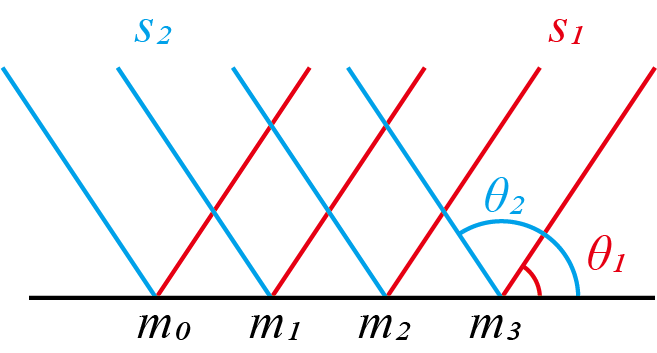
\includegraphics[width = 0.4\textwidth]{pic/pic1.png}
        \end{figure}

        First we take the Fourier Transforms of the sources signals and the received signals.

        $$
        s(t) \stackrel{FFT}{\Longrightarrow} S(f) \qquad x(t) \stackrel{FFT}{\Longrightarrow} X(f)
        $$

        If the AoA between of source 1 and source 2 are $\theta_1 ,\, \theta_2$, then the delay is $\phi_1 = \frac{2\pi d cos(\theta_1)f_ik}{c},\, \phi_2 = \frac{2\pi d cos(\theta_2)f_ik}{c},\, k = 0,1,2,3$
        
        So the received signals can be written as 
        $$
        \left[\begin{matrix}X_0\\X_1\\X_2\\X_3\\\end{matrix}\right]=\left[\begin{matrix}e^0&e^0\\e^{j\phi_1}&e^{j\phi_2}\\e^{j{2\phi}_1}&e^{j{2\phi}_2}\\e^{j{3\phi}_1}&e^{j{3\phi}_2}\\\end{matrix}\right]\left[\begin{matrix}S_1\\S_2\\\end{matrix}\right]
        $$
        
        The purpose of the part 4 is to solve $S_1$ and $S_2$. According to the previous part, we already get $\theta_1$ and $\theta_2$ by AoA estimation, and then we preceed as follows.
        $$
        \begin{aligned}
        &\left[\begin{matrix}e^0&e^{-j\phi_1}&e^{-j\phi_2}&e^{-j\phi_3}\\\end{matrix}\right]
        \left[\begin{matrix}X_0\\X_1\\X_2\\X_3\\\end{matrix}\right]
        =
        \left[\begin{matrix}e^0&e^{-j\phi_1}&e^{-j\phi_2}&e^{-j\phi_3}\\\end{matrix}\right]
        \left[\begin{matrix}e^0&e^0\\e^{j\phi_1}&e^{j\phi_2}\\e^{j{2\phi}_1}&e^{j{2\phi}_2}\\e^{j{3\phi}_1}&e^{j{3\phi}_2}\\\end{matrix}\right]
        \left[\begin{matrix}S_1\\S_2\\\end{matrix}\right]\\
        &=4S_1 + \sum_{k=1}^{3} e^{j k\left(\phi_{2}-\phi_{1}\right)} S_{2}\\
        &\approx  4S_1
        \end{aligned}
        $$

        Thus we successfully separate S1 and in the same way we can separate S2.

        $$\begin{aligned}
        S_1(f_i) & \approx  \frac{1}{4} \left[\begin{matrix}e^0 & e^{-j\frac{2\pi d cos(\theta_1)1f_i}{c}}& e^{-j\frac{2\pi d cos(\theta_1)2f_i}{c}}& e^{-j\frac{2\pi d cos(\theta_1)3f_i}{c}}
        \end{matrix}\right] \left[\begin{matrix}
            X_0(f_i) \\
            X_1(f_i) \\
            X_2(f_i) \\
            X_3(f_i) 
        \end{matrix}\right]\\
        & \approx   \frac{1}{4} \sum_{k=0}^{3}e^{-j\frac{2\pi d cos(\theta_1)f_ik}{c}}\cdot X_k(f_i)
        \end{aligned}$$

        Finally, we take the inverse Fourier transform of $S_1$ and $S_2$ to complete the separation.

        $$
        S(f) \stackrel{IFFT}{\Longrightarrow} s(t)
        $$

    \section{Results}
        \subsection{Part 1 and Part 2}
        \begin{figure}[H]
            \centering
            \begin{minipage}{0.49\linewidth}
                \centering
                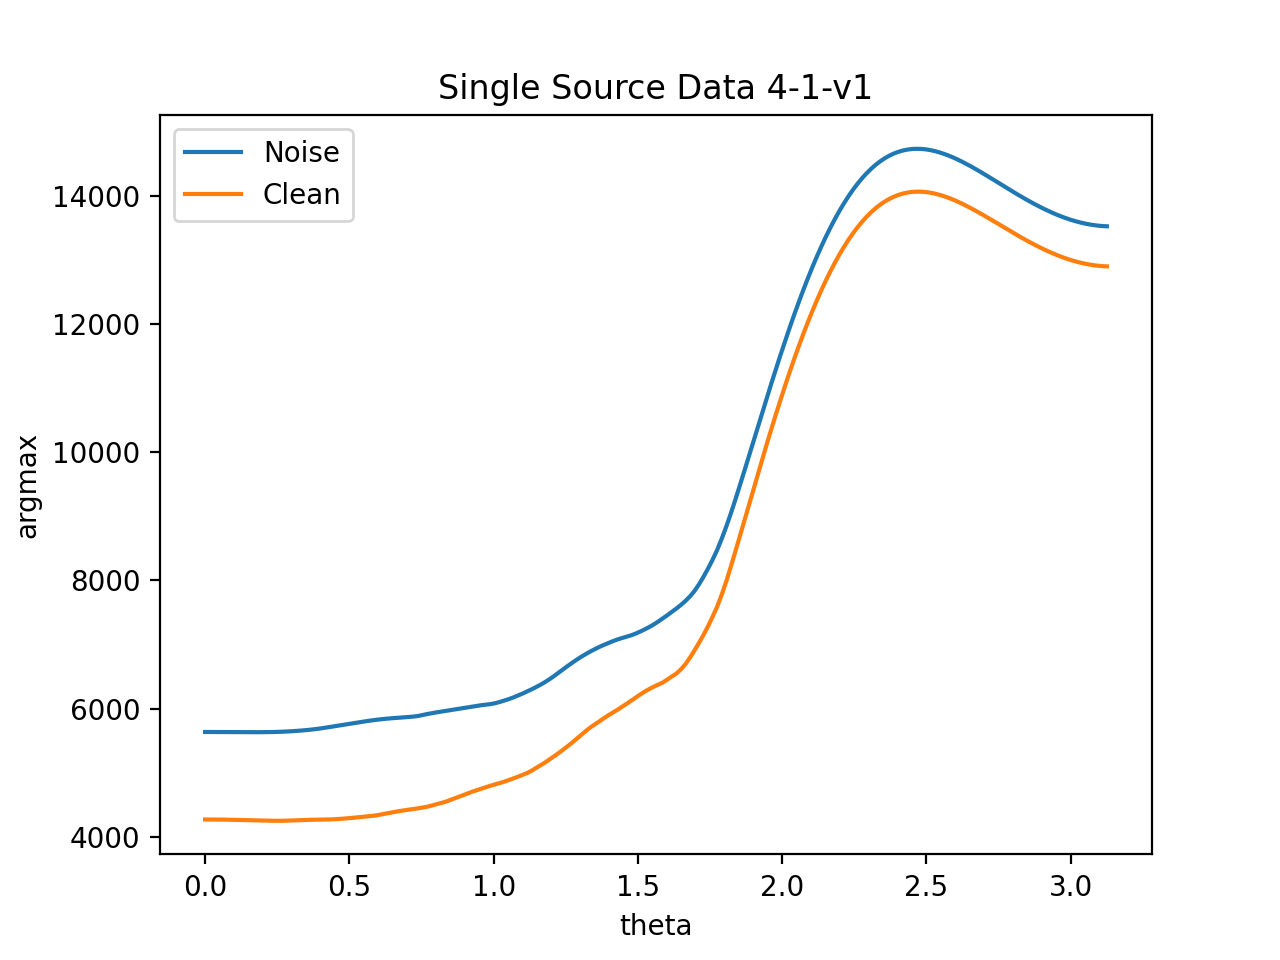
\includegraphics[width=0.9\linewidth]{pic/Figure_1.png}
                \caption{4-1-v1}
            \end{minipage}
            \begin{minipage}{0.49\linewidth}
                \centering
                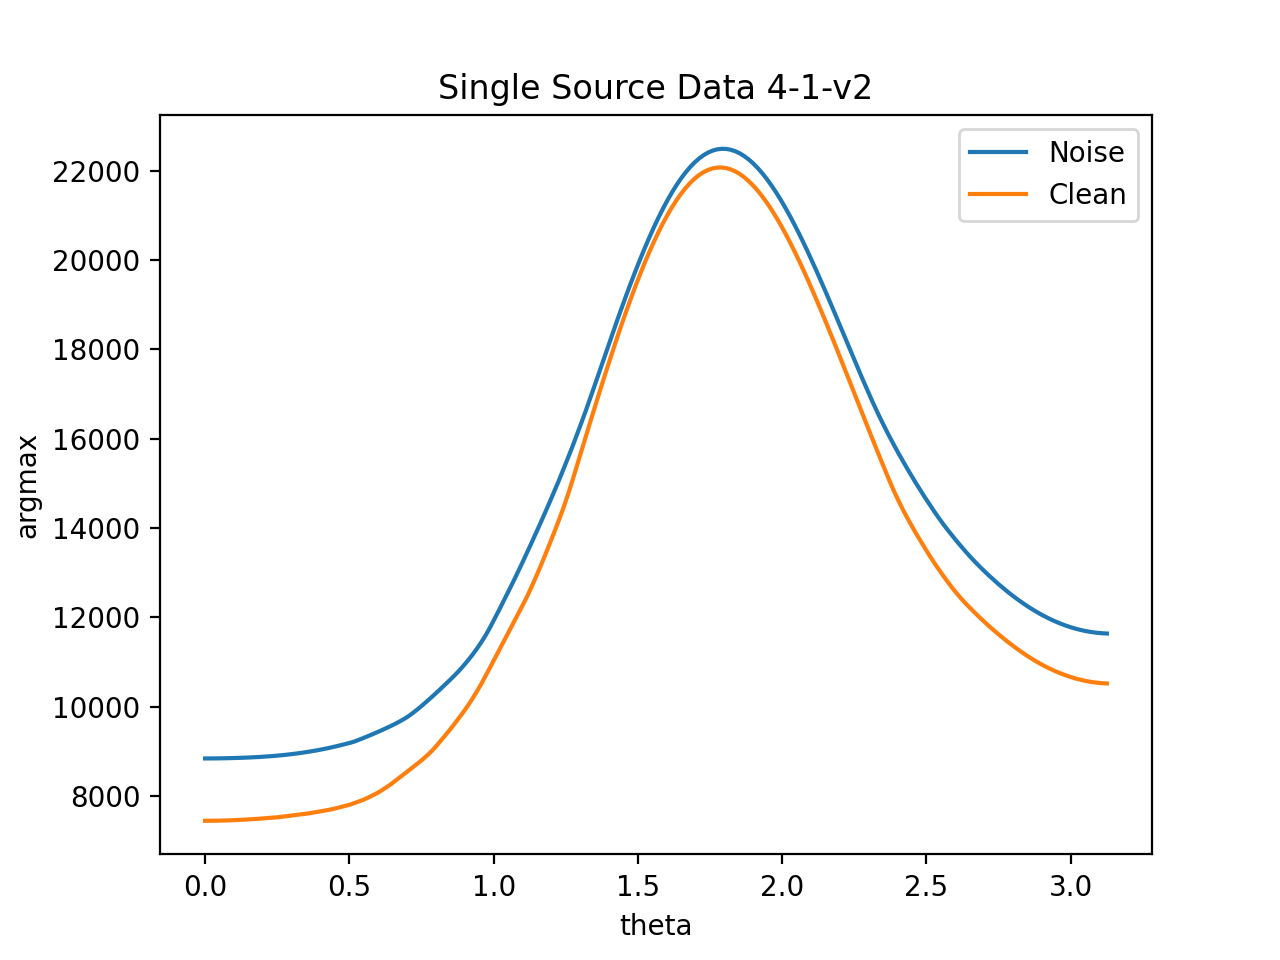
\includegraphics[width=0.9\linewidth]{pic/Figure_2.png}
                \caption{4-1-v2}
            \end{minipage}
            %\qquad
            
            \begin{minipage}{0.49\linewidth}
                \centering
                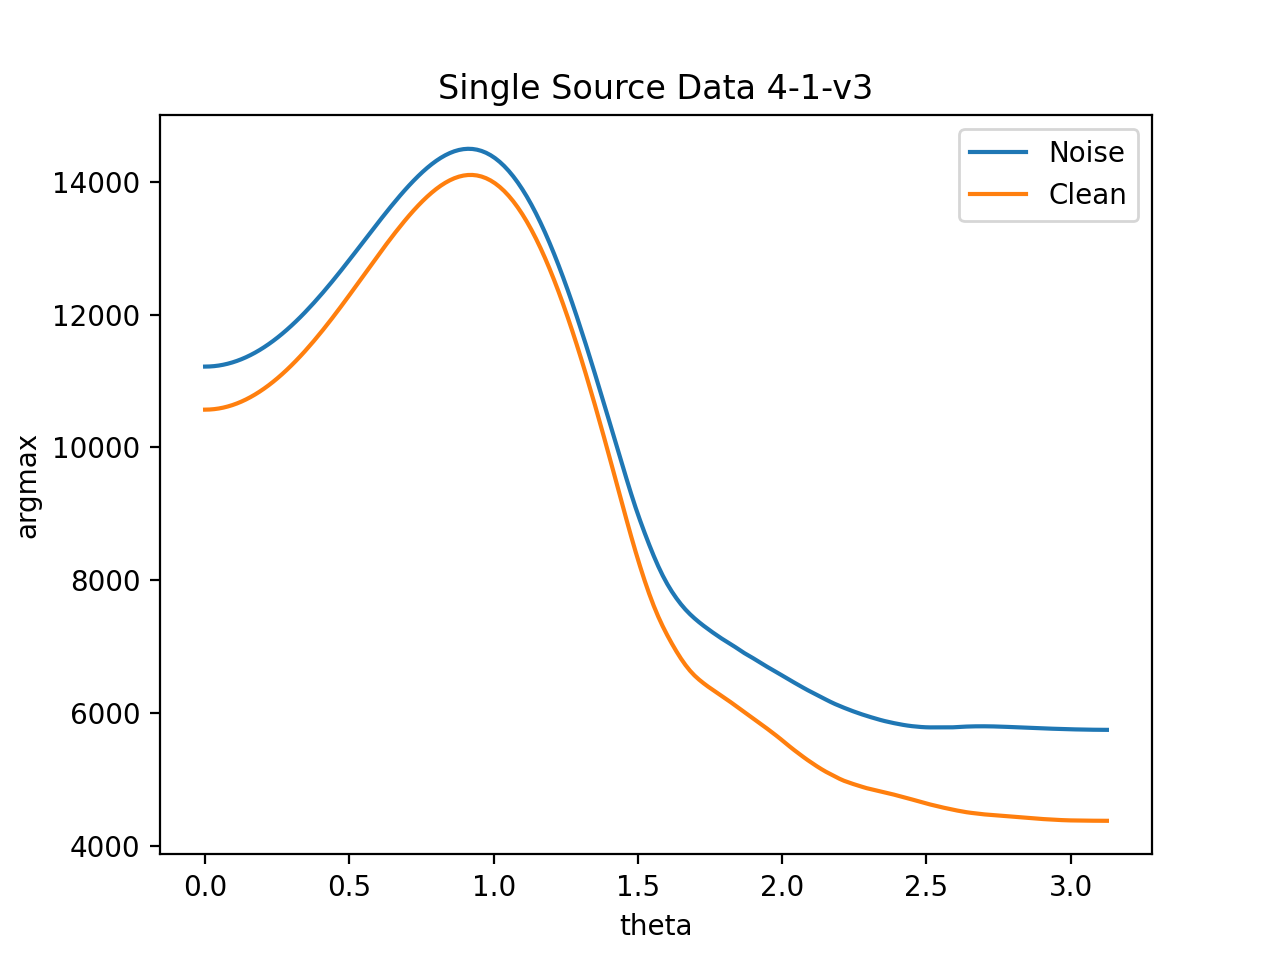
\includegraphics[width=0.9\linewidth]{pic/Figure_3.png}
                \caption{4-1-v3}
            \end{minipage}
            \begin{minipage}{0.49\linewidth}
                \centering
                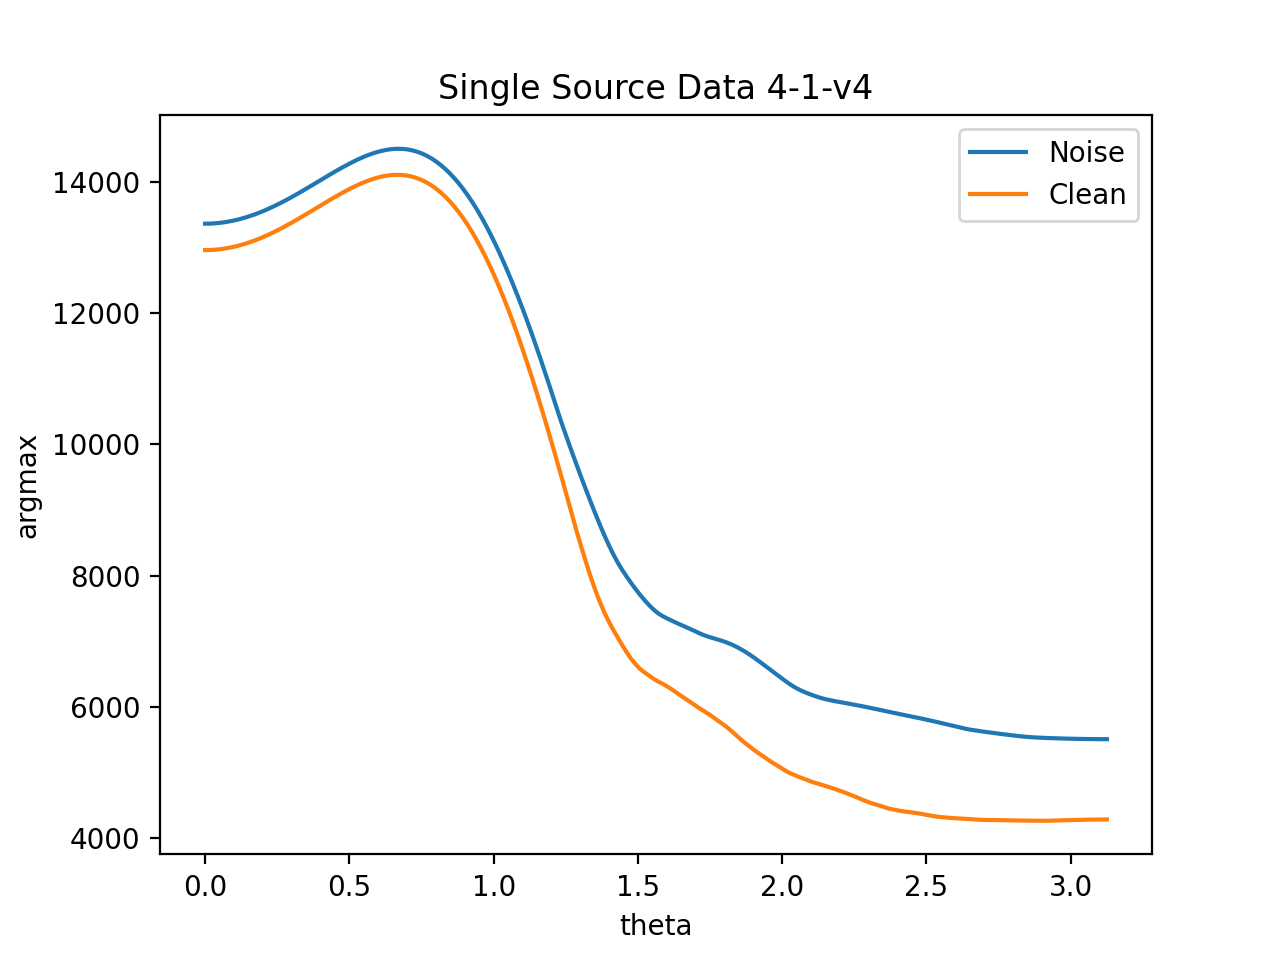
\includegraphics[width=0.9\linewidth]{pic/Figure_4.png}
                \caption{4-1-v4}
            \end{minipage}
        \end{figure}

        And the estimated AoA of each part is 

        \begin{table}[H]
            \centering
            \begin{tabular}{@{}ccccc@{}}
            \toprule
                  & v1    & v2    & v3    & v4    \\ \midrule
            Clean & 2.466 & 1.791 & 0.927 & 0.660 \\
            Noise & 2.466 & 1.791 & 0.911 & 0.675 \\ \bottomrule
            \end{tabular}
        \end{table}
    
        \subsection{Part 3}
        \begin{figure}[H]
            \centering
            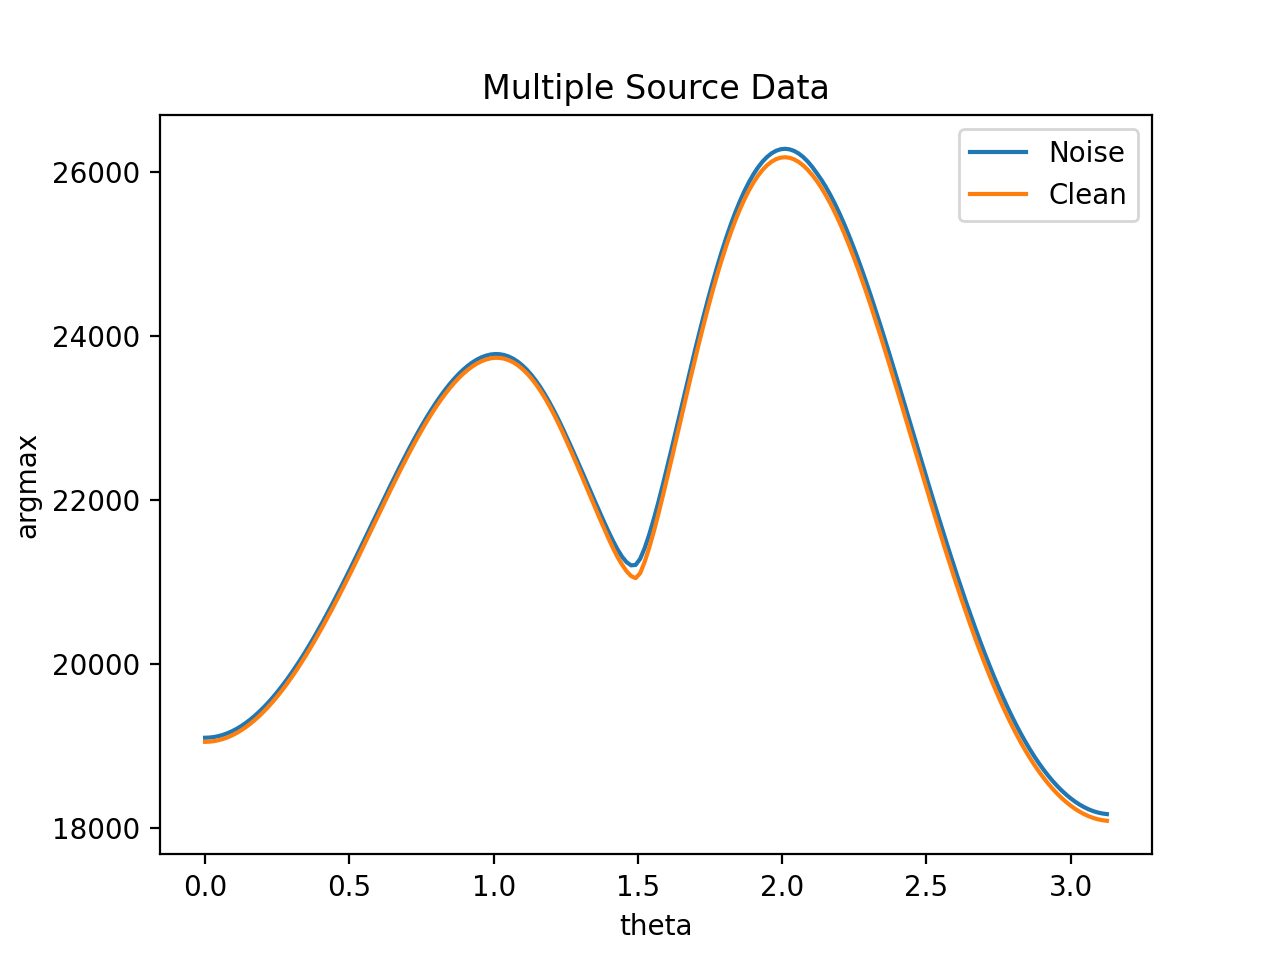
\includegraphics[width = 0.5\textwidth]{pic/Figure_5.png}
            \caption{Multiple Source Data}
        \end{figure}

        And the estimated AoA is 

        % Please add the following required packages to your document preamble:

        \begin{table}[H]
            \centering
            \begin{tabular}{@{}ccc@{}}
            \toprule
                & source 1 & source 2 \\ \midrule
            Clean & 1.005    & 2.011    \\
            Noise & 1.005    & 2.011    \\ \bottomrule
            \end{tabular}
        \end{table}



\end{document}